
\documentclass{article}
\usepackage[utf8]{inputenc}

\usepackage{amsthm}
\usepackage{amsmath}
\newtheoremstyle{mystyle}% name
  {\topsep}% Space above
  {\topsep}% Space below
  {\normalfont}% Body font
  {}% Indent amount
  {\bfseries}% Theorem head font
  {}%Punctuation after theorem head
  {.5em}%Space after theorem head
  {}% theorem head spec
\theoremstyle{mystyle}
\newtheorem{prob}{Problem}
\usepackage{graphicx}
\usepackage{wrapfig}


\title{EN.520.216 Homework 1}
\author{LJ Gonzales}
\date{February 2023}

\begin{document}
\maketitle
\section{Manufacturing Problems}
\begin{prob}
\begin{enumerate} 
	\item On the wafer "length" of 36L, we can have at most $\lfloor\frac{3}{36\times90\times10^9/2}\rfloor=1851$ "rows" of transistors and $\lfloor\frac{3}{24\times90\times10^9/2}\rfloor=2777$ "columns", for a total of 5,140,227 transistors. This makes the assumption that transistors are allowed to be side-to-side with no space between them (or that the necessary space is included in the provided area). Also, we assume the chip is single-layer.
\item Same as the previous, 5144032, with the added assumption that both nmos and pmos types are made to be the same size, which would probably not be the case.
\item 
\end{enumerate}
\end{prob}

\section{Device Physics Problems}
\begin{prob}
\begin{enumerate}
    \item The Fermi function gives the probability that a state \emph{at a given energy} is filled with an electron. Because the total amount of available states at a given energy is large, this is basically equivalent to the fraction of states that are filled by an electron.
    \item We use the Fermi function \[f(E)=\frac{1}{1+e^{(E-E_f)/kT}}\] with $E=E_f+0.225kT$, giving $\frac{1}{1+e^{0.225}}\approx0.444$.
    \item Here $E>>E_f$ so we consider that most of the states at this level are empty.
\end{enumerate}
\end{prob}

\begin{prob}
	We know that $n_i\approx\int_{E_c}^{\infty}g(E)e^{\frac{E-E_{fi}}{kT}}dE$ and $n_d\approx\int_{E_c}^{\infty}g(E)e^{\frac{E-E_{fd}}{kT}}dE$. But now if we just call $E_{fd}=E_{fi}+\Delta E$ where E is just some constant that represents how far the doped fermi level is relative to the intrinsic fermi level, we find that:  
	\[\begin{split} 
		\frac{n_i}{n_d}=\frac{\int_{E_c}^{\infty}g(E)e^{\frac{E-E_{fi}}{kT}}dE}{\int_{E_c}^{\infty}g(E)e^{\frac{E-(E_{fi}+\Delta E)}{kT}}dE} \\
    =\frac{1}{e^{- \Delta E/kT}}\frac{\int_{E_c}^{\infty}g(E)e^{\frac{E-E_{fi}}{kT}}dE}{\int_{E_c}^{\infty}g(E)e^{\frac{E-E_{fi}}{kT}}dE}=\frac{1}{e^{-\Delta E/kT}} \\
 \therefore \ln{\frac{10^{10}}{10^{17}}} = \frac{-\Delta E}{kt} \\
	\end{split} 
 \]
 \end{prob}

From this we substitute our known values of k and T, $8.6\times10^{-5}$ and $295$, respectively, to find that $\Delta E\approx0.409$, in other words the Fermi level is 0.409eV above the intrinsic fermi level of 1.1eV, for a total of about 1.5eV. 

\begin{prob}
    \begin{enumerate}
        \item 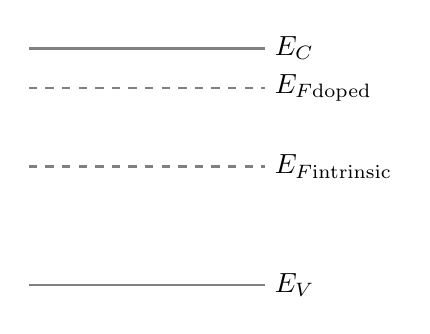
\begin{tikzpicture}
        \draw[gray, thick] (-1,3) -- (2,3);
        \node[right] at (2,3) {$E_C$};
        \draw[gray, thick, dashed] (-1,2.5) -- (2,2.5);
        \node[right] at (2,2.5) {$E_{F\text{doped}}$};
        \draw[gray, thick, dashed] (-1,1.5) -- (2,1.5);
        \node[right] at (2,1.5) {$E_{F\text{intrinsic}}$};
        \draw[gray, thick] (-1,0) -- (2,0);
        \node[right] at (2,0) {$E_V$};
        \end{tikzpicture}

        \item The acceptor concentration can be calculated from the additional assumption $p=N_A$ and the law of mass action $np=n_i^2$, such that $N_A=p=\frac{(10^{10})^2}{10^{17}}=10^3$ acceptors/cm3
    \end{enumerate}
\end{prob}

\begin{prob}
\begin{enumerate}
    \item With a similar calculation used in the previous problem, we find \[\begin{split}
    E_g=-(2\times8.6\times10^{-5}\times300)\ln(\frac{10^{13}}{5.2\times10^{15}\times300^{3/2}})
    \end{split}\]
    \item Here we need to first find the concentration of electrons as a result of this doping before inserting in the same equation. We find that $n=\frac{n_i^2}{N_A}=\frac{(10^{10})^2}{5\times10^{14}}=0.2\times10^6$ hence:
    \[\begin{split}
    E_g=-(2\times8.6\times10^{-5}\times300)\ln(\frac{0.2\times10^6}{5.2\times10^{15}\times300^{3/2}})
    \end{split}\]
\end{enumerate}
\end{prob}

\end{document}
